\documentclass[letterpaper, 10 pt, conference]{ieeeconf}  
\usepackage{amsfonts, amssymb}
\usepackage{array}
\usepackage{graphicx}
\usepackage{multirow}
%\usepackage{float} 
\usepackage{subcaption}
%============================================================================================
% Math symbols
\newcommand \Rbb{\mathbb{R}}
%\newcommand \coloneqq{:=} defined in mathtools package
\newcommand \supp{\textup{supp}}
\newcommand \Supp[1]{ \supp \left( #1 \right) }
\newcommand \eqDef{\overset{\Delta}{=}}

\newcommand \vect[1]{\boldsymbol #1}
\newcommand \qed {\begin{flushright} $\blacksquare$ \end{flushright}}
%============================================================================================
% Variables 
\newcommand \flow{x}
\newcommand \flowV{\vect \flow}
\newcommand \flowMax{\flow^{\max}}
\newcommand \mode{m}
\newcommand \modeV{\vect \mode}

\newcommand \mass{\rho}
\newcommand \massMax{\mass^{\max}}
\newcommand \massCrit{\mass^{\text{crit}}}

\newcommand \speedFF{v^{f}}
\newcommand \speedCong{v^{c}}

%============================================================================================
% Parameters
\newcommand \length{L}
\newcommand \NLinks{N}
\newcommand \compRate{\alpha}
\newcommand \cR{\compRate}
\newcommand \demand{r}
\newcommand \demandMax[1]{\demand^{\textup{NE}} ( #1 ) }
\newcommand \parA{a}

%============================================================================================
% Notation
\newcommand \link{n}

% Stackelberg thresholds notation
\newcommand \lastNash[1]{b(#1)}
\newcommand \lastStack[1]{l(#1)}
\newcommand \lastNC[1]{k(#1)}
\newcommand \selfish[1]{\demand_{#1}}
\newcommand \cardNash{c}
\newcommand \maxR[1]{\demandMax{k_{#1}}}
% 

\newcommand \cFlow[2]{ \hat{\flow}_{#1} ( #2 ) }
\newcommand \ffNashMode[1]{ \modeV^{#1}}
\newcommand \ffNashFlow[2]{\flowV^{#1,#2}}

\newcommand \stackFlow{s}
\newcommand \sV{\vect \stackFlow}
\newcommand \respFlow{t}
\newcommand \tV{\vect \respFlow}
\newcommand \epsV{\vect \epsilon}


\newcommand \latency{\ell}
\newcommand \latencyMass{\latency^{\mass}}
\newcommand \totalLatency{C}
\newcommand \massCongFunc{\mass^{\text{cong}}}

\newcommand \BNE[2]{\textup{BNE} (#1, #2) }
\newcommand \NE[2]{\textup{NE} (#1, #2) }
\newcommand \NEf[2]{\textup{NE}_\textup{f} (#1, #2) }
\newcommand \NEc[2]{\textup{NE}_\textup{c} (#1, #2) }
\newcommand \NCF[3]{\textup{NCF} (#1, #2, #3) }
\newcommand \stackSet[3]{\textup{S} (#1, #2, #3) }
\newcommand \stackSetOpt[3]{\textup{S}^\star (#1, #2, #3) }
\newcommand \POS[3]{\textup{POS} (#1,#2, #3)}
\newcommand \SO[2]{\textup{SO} (#1,#2)}

\newcommand \std[1] {#1{\NLinks}{\demand}}
\newcommand \stdStack[1]{#1{\NLinks}{\demand}{\compRate}}


%============================================================================================
% over braces and under braces
\usepackage{mathtools}

\newcommand \overbrac[3]{
\overbracket{\vphantom{#1} #2}^{\mathclap{#3}}
}
\newcommand \underbrac[3]{
\underbracket{\vphantom{#1} #2}_{\mathclap{#3}}
}

\newcommand \overbracBig[2]{
\overbrac{\Big(}{#1}{#2}
}
\newcommand \underbracBig[2]{
\underbrac{\Big(}{#1}{#2}
}

\newcommand \overbracbig[2]{
\overbrac{\big(}{#1}{#2}
}
\newcommand \underbracbig[2]{
\underbrac{\big(}{#1}{#2}
}

%-----------------------------------------------------------------------------------------------------------------------------------------------------------------
% some definitions for the table
\newcommand{\vcell}[2][c]{
\begin{tabular}[t]{@{}p{#1}@{}}
#2
\end{tabular}
}

\def \bul{$\centerdot$ }

%-----------------------------------------------------------------------------------------------------------------------------------------------------------------





\IEEEoverridecommandlockouts
\overrideIEEEmargins

%-----------------------------------------------------------------------------------------------------------------------------------------------------------------
% environments and commands

\newtheorem{definition}{Definition}
\newtheorem{lemma}{Lemma}
\newtheorem{theorem}{Theorem}
\newtheorem{proposition}{Proposition}
\newtheorem{corollary}{Corollary}
\newtheorem{remark}{Remark}

%%%%%%%%%%%%%%%%%%%%%%%%%%%%%%%%%%%%%%%%%%%%%%%%%%%%%%%%%%%%%%%%%%%%%%%%%%%%%%%%


\begin{document}

\author{Yasser Jebbari \and Walid Krichene \and Jack D. Reilly \and Alexandre M. Bayen}% <-this % stops a space
\title{Stackelberg Thresholds on Parallel Networks with Horizontal Queues}

\maketitle

\thispagestyle{empty}
\pagestyle{empty}

%%%%%%%%%%%%%%%%%%%%%%%%%%%%%%%%%%%%%%%%%%%%%%%%%%%%%%%%%%%%%%%%%%%%%%%%%%%%%%%%
% !TEX root = stack-thresh.tex

\begin{abstract}
We study Stackelberg routing games on parallel networks with horizontal queues, in which a coordinator (leader) controls a fraction $\compRate$ of the total flow on the network, and the remaining players (followers) choose their routes selfishly. The objective of the coordinator is to minimize a system-wide cost function, the total travel-time, while anticipating the response of the followers. 

Nash equilibria of the routing game (with zero control) are known to be inefficient in the sense that the total travel-time is sub-optimal. Increasing the \emph{compliance rate}~$\compRate$ improves the cost of the equilibrium, and we are interested in particular in the \emph{Stackelberg threshold}, i.e. the minimal compliance rate that achieves a \emph{strict} improvement. In this work, we derive the optimal Stackelberg cost as a function of the compliance rate~$\compRate$, and obtain, in particular, the expression of the Stackelberg threshold.
\end{abstract}


%%%%%%%%%%%%%%%%%%%%%%%%%%%%%%%%%%%%%%%%%%%%%%%%%%%%%%%%%%%%%%%%%%%%%%%%%%%%%%%%
\section{Introduction}
\label{sec:intro}

\subsection{Motivation and related work}

Non-cooperative network routing games model the interaction of selfish network users. Each player chooses a route that  minimizes their individual travel-time. A Nash equilibrium, or Wardrop equilibrium~\cite{wardrop1952some}, is a route assignment in which each player cannot improve their individual travel-time by unilaterally switching their route. The system-wide cost of a Nash equilibrium is, in general, sub-optimal, i.e. worse than the cost of the social optimum where a central coordinator assigns routes to every player in order to minimize the total cost \cite{roughgarden2002bad}.

In order to \textit{cope with selfishness}, i.e. to reduce the cost of Nash equilibria, different tools have been studied, including congestion pricing~\cite{Ozdaglar2007}, capacity allocation~\cite{Korilis97capacityallocation} and Stackelberg routing~\cite{roughgarden2001stackelberg,aswani2011game,DBLP:conf/soda/Swamy07,Korilis97achievingnetwork}. In the Stackelberg routing game, a fraction~$\compRate$ of the players are assumed to be controlled by a central coordinator. This may be the case in several situations, for instance when some players are not selfish and care about the system-wide efficiency, or when they have external incentive to do so. The total flow of these players will be referred to as  \emph{compliant flow}, and their routes are assigned by the central coordinator. The objective of the coordinator is to minimize the total travel-time, while anticipating the response of the remaining players, referred to as \emph{non-compliant}. The solution reached in this case is a Stackelberg equilibrium.

In a Stackelberg routing game, the system-wide cost is a non-increasing function of the compliance rate $\compRate$. When $\compRate = 0$, the coordinator has no control, and the equilibrium is simply a Nash equilibrium. The cost is then maximal. When $\compRate = 1$, the coordinator has total control, the cost is minimal, and the equilibrium is by definition, the social optimum.

Although the cost of the equilibrium is a non-increasing function of $\compRate$, it may not be \emph{strictly decreasing}. In particular, if the fraction of controlled players is too small, there may be no improvement. This leads to the following question: what is the minimal compliance rate\footnote{We observe that the Stackelberg threshold is only defined when the cost of the social optimum is strictly less than the cost of a Nash equilibrium.} needed in order to achieve strict improvement in the total cost? This minimal fraction is called \textit{Stackelberg threshold} \cite{Sharma07stackelbergthresholds}. Computing Stackelberg thresholds is of practical importance in several situations, such as traffic planning and control~\cite{krichene12}.


In this paper, we consider the same setting as in~\cite{krichene12}, i.e. parallel networks with horizontal queues. In this setting, the latency of each link is given by a function that satisfies the assumptions of the HQSF  latency class (horizontal queues, singled-valued in free-flow). This class is useful in modeling congestion due to horizontal queues, e.g. in a transportation network, as opposed to vertical queues, e.g. in a communication network.

We derive the expression of optimal Stackelberg cost for the HQSF class on parallel networks. In particular, we obtain an expression for Stackelberg thresholds.

%The main idea comes from the observation that the cost of a Nash equilibrium does not depend directly on the demand $r$, but on an effective demand that is denoted $\demandMax{\lastNash{r}}$. Thus, there is an actual improvement if and only if the amount of compliant users is enough to decrease the effective demand of selfish players. 

%-----------------------------------------------------------------------------------------------------------------------------------------------------------------
\subsection{Organization of the article}

In Section~\ref{sec:previous}, we define the Stackelberg routing game, present the assumptions of the model (in particular the latency functions) and review previous results. In Section~\ref{sec:support}, we characterize the supports of Nash equilibria and Stackelberg equilibria, then derive in Section~\ref{sec:cost} the general expression of the optimal Stackelberg cost. This leads in particular to the expression of Stackelberg thresholds, given in Section~\ref{sec:threshold}. Finally, we present some numerical results in Section~\ref{sec:numerical}.




% !TEX root = stack-thresh.tex

\section{Definitions and previous results}
\label{sec:previous}

In this section we present the problem setting and review previous results for Stackelberg routing on parallel networks with horizontal queues~\cite{krichene12}.




%-----------------------------------------------------------------------------------------------------------------------------------------------------------------
\subsection{Routing game on a parallel link with horizontal queues}
\label{sec:previous-Nash}

We consider a non-atomic routing game on a network of~$\NLinks$ parallel links, subject to flow demand~$\demand$ (see Figure~\ref{fig:network}). Each non-atomic player chooses a link ${n \in \{1, \dots, N\} }$ that minimizes their individual travel time, or latency, given by a function $\latency_n(\flow_n, \mode_n)$ of the total flow $\flow_n \in [0, \flowMax_n]$ and the congestion state $\mode_n \in \{0,1\}$ on the link. Here the latency on a link $n$ depends not only on the flow $\flow_n$, but on the congestion state of the link as well. By definition, the congestion state specifies whether the link is in free-flow $(\mode_n = 0)$ or is congested $(\mode_n = 1)$.
%
\begin{figure}[h]
\centering
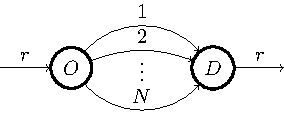
\includegraphics{TikZ/parallel_network.pdf}
\caption{Parallel network with $\NLinks$ links and demand~$\demand$.}
\label{fig:network}
\end{figure}
%
The latency functions are assumed to be in the HQSF class (horizontal queues, single-valued in free-flow) \cite{krichene12}, i.e. satisfies the following assumptions:
\begin{enumerate}
\item The latency in free-flow ${ \latency_n(\cdot, 0): [0, \flowMax_n] \rightarrow \Rbb_+ }$ is single-valued. We will denote by $a_n$ its value, called the \emph{free-flow latency}.
\item The latency in congestion $ \latency_n(\cdot, 1) : (0, \flowMax_n) \rightarrow (a_n, +\infty) $ is continuous decreasing.
\item Continuity: ${\lim_{\flow_n \rightarrow \flowMax_n} \latency(\flow_n, 1) = \latency_n(\flowMax_n, 0) = a_n}$
\end{enumerate}
We also assume that the free-flow latencies are distinct, and that the links are ordered by increasing free-flow latency, i.e.
\begin{equation}
\label{eq:index}
a_1 < a_2 < \dots < a_\NLinks
\end{equation}

Let $(\NLinks, \demand)$ denote an instance of the routing game, $\flowV \in \mathbb{R}_+^\NLinks$ the vector of flows, $\flowV^{\max} \in \Rbb_+^\NLinks$ the vector of capacities, and $\modeV \in \{0,1\}^\NLinks$ the vector of congestion states on the network. The assignment $(\flowV, \modeV)$ is said to be a feasible assignment if for every link $n$, the flow $\flow_n$ is admissible ($\flow_n \leq \flowMax_n$) and the total flow is conserved, i.e. $\sum_{n=1}^{\NLinks} \flow_n = \demand$. For a feasible assignment $(\flowV, \modeV)$, we define the total cost $C(\flowV, \modeV)$ as the sum of the latencies experienced by all users on all links
\[
C(\flowV, \modeV) = \sum_{n=1}^\NLinks {\latency_n(\flow_n, \mode_n) \flow_n}
\]

Let $\Supp{\flowV} = \{ n \in \{1, \dots, \NLinks\} | \flow_n > 0\}$ denote the support of a flow vector~$\flowV$.
\begin{definition}\emph{Nash equilibrium}\\
\label{def:NashEq}
A feasible assignment $(\flowV, \modeV)$ for the instance $(\NLinks, \demand)$ is a Nash equilibrium if there exists a positive latency $\latency_0 > 0$ such that
\begin{equation}
\begin{aligned}
n \in \Supp{\flowV} \Rightarrow \latency_n(\flow_n, \mode_n) = \latency_0 \\
n \notin \Supp{\flowV} \Rightarrow \latency_n(\flow_n, \mode_n) \geq \latency_0
\end{aligned}
\end{equation}
This means in particular that every user is experiencing the same travel time $\latency_0$. In this case the total cost of the equilibrium is simply~$C(\flowV, \modeV) = \demand \latency_0$. We will denote by $\std\NE$ the set of Nash equilibria of the instance $(\NLinks, \demand)$.
\end{definition}

\begin{definition}{\emph{Single-link free-flow equilibria and congestion flows}\\}
\label{def:CongFlow}
Let $(\flowV, \modeV) \in \std\NE$ be a Nash equilibrium, and let $k = \max \Supp{\flowV}$ be the last link (i.e. the one with the largest free-flow latency) in the support of~$\flowV$. If link $k$ is in free-flow, then $(\flowV, \modeV)$ is said to be a single-link-free-flow equilibrium, and satisfies the following properties:
\begin{itemize}
\item $\Supp{\flowV} = \{1, \dots, k\}$
\item The common latency on the support of~$\flowV$ is $a_k$
\item The flow on links $n \in \{1, \dots, k-1\}$ is given by the congestion flows $\cFlow{n}{k}$ defined by
\[
\cFlow{n}{k} = \latency_n(.,1)^{-1}(a_k)
\]
\end{itemize}
Therefore a single-link-free-flow equilibrium is of the form
\begin{align*}
\modeV &= (1, \dots, 1, \overbracBig{0}{k}, \dots, 0) \\
\flowV &= \big( \cFlow{1}{k}, \dots, \cFlow{k-1}{k}, \overbracBig{\demand - \sum_{n=1}^{k-1}\cFlow{n}{k}}{k}, 0, \dots, 0 \big)
\end{align*}
\end{definition}

Figure~\ref{fig:ff_nash} shows an example of a single-link-free-flow equilibrium on an instance with $\NLinks = 4$ links. We observe that the congestion flow $\cFlow{n}{k}$ is a decreasing function of $k$ since $k \mapsto a_k$ is increasing by assumption~\eqref{eq:index} and $\latency_n(\cdot, 1)$ is decreasing.
%%%
\begin{figure}[h]
\centering
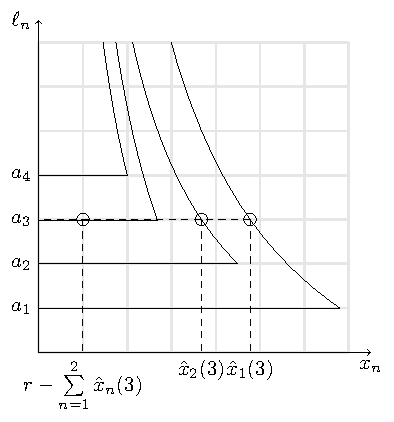
\includegraphics[width=2.5in]{TikZ/ff_nash.pdf}
\caption{Example of a single-link-free-flow equilibrium.}
\label{fig:ff_nash}
\end{figure}
%

\begin{definition}
\label{def:maxDemand}
We denote, for any $k\in \{1,\ldots,N\}$, by $\demandMax{k}$ the maximum demand such that the set of Nash equilibria $\NE{k}{\demand}$ is non-empty. It is given by
\begin{equation}
\demandMax{k} = \max_{ j \in \{1,\dots, k\} } \{\flowMax_j + \sum_{n=1}^{j-1} \cFlow{n}{j} \}
\end{equation}
\end{definition}

\begin{remark}
\label{remark:maxDemand}
We also have the following property: a single-link-free-flow equilibrium exists for the instance $(k, \demand)$ if and only if $\demand \leq \demandMax{k}$.
\end{remark}

Proofs of these facts are given in Lemma~1 and Corollary~2 in~\cite{krichene12}, and they are provided in the Appendix for completeness. By definition, we have $\forall k \in \{2, \dots, \NLinks \}$, ${ \demandMax{k} \geq \demandMax{k-1} }$. We will be interested, in particular, in links that strictly increase the maximum demand, i.e. such that $\demandMax{k} > \demandMax{k-1}$. We denote these links by $k_1, \dots, k_c$, defined by induction as follows:
\begin{align}
& k_1 = 1 \\
& \forall i \in \{2, \dots, c\}, \ k_{i} = \min \{n \leq \NLinks | \demandMax{n} > \demandMax{k_{i-1}}\} \label{eq:nj}
\end{align}
Therefore we have
\[
\demandMax{1} = \demandMax{k_1} < \dots < \demandMax{k_c} = \demandMax{\NLinks}
\]
Here $c$ is the number of distinct elements in the set $\{\demandMax{k}, k \in \{1, \dots, \NLinks\}\}$.


\begin{definition}{\emph{Best Nash equilibrium}\\}
\label{def:BstNashEq}
The set of best Nash equilibria is the set of Nash equilibria that minimize the system-wide latency. 
\begin{equation}
\std \BNE = \underset{(\flowV, \modeV) \in \std\NE}{\arg\min} C(\flowV, \modeV)
\end{equation}
\end{definition}

\begin{remark}
\label{remark:smallest-support}
It is shown in~\cite{krichene12} (Lemma~3) that the best Nash equilibrium is unique, and that it is equal to the single-link-free-flow equilibrium with smallest support. With a slight abuse of notation, we will use $\std \BNE$ to denote the unique best Nash equilibrium (identifying the set with its unique element).
\end{remark}

\begin{proposition}\emph{Last link in the support of a best Nash equilibrium}\\
\label{prop:lastNash}
Let $(\flowV, \modeV)$ be the best Nash equilibrium for the instance $(\NLinks, \demand)$, then the last link in the support of~$\flowV$ is given by
\begin{equation}
\max \Supp{\flowV} = \min \left\{k: r \leq \demandMax{k} \right\}
\end{equation}
\end{proposition}

\begin{proof}
Let $b = \max \Supp{\flowV}$. Since an equilibrium exists for the instance~$(b, \demand)$, then $\demand \leq \demandMax{b}$ by Definition~\ref{def:maxDemand} of the maximum demand. And for all $k$ such that $\demand \leq \demandMax{k}$, by Remark~\ref{remark:maxDemand}, there exists a single-link-free-flow equilibrium supported on  $\{1, \dots, k\}$, thus by Remark~\ref{remark:smallest-support}, $k \geq b$. Therefore $b$ is the minimum such index.
\end{proof}

%-----------------------------------------------------------------------------------------------------------------------------------------------------------------
\subsection{Stackelberg routing game}
\label{sec:previous-Stack}

In the Stackelberg routing game, a central coordinator controls a fixed fraction of the total flow. This~\emph{compliant flow} corresponds to players who are either altruistic and care about the system-wide latency, or who may have an external incentive to be controlled by the coordinator. First, the coordinator (the leader) chooses the routes of the compliant flow. The resulting vector of flows is called a Stackelberg strategy and denoted by $\sV$. It satisfies $\sum_{n = 1}^\NLinks s_n = \compRate \demand$. Then the strategy $\sV$ of the leader is revealed, and the remaining players (the followers, corresponding to non-compliant flow $(1-\compRate) \demand$) choose their routes selfishly. The resulting non-compliant assignment, \emph{induced} by Stackelberg strategy~$\sV$, is denoted by $(\tV(\sV), \modeV(\sV))$. It is assumed to be the best Nash equilibrium \cite{krichene12} and satisfies the following: there exists a common latency $\latency_0$ on the support of $\tV(\sV)$ such that
\begin{equation}
\label{eq:induced_eq}
\begin{aligned}
n \in \Supp{\tV(\sV)} &\Rightarrow \latency_n(t_n(\sV) + s_n, \mode_n(\sV)) = \latency_0 \\
n \notin \Supp{\tV(\sV)} &\Rightarrow \latency_n(s_n, \mode_n(\sV)) \geq \latency_0
\end{aligned}
\end{equation}

We will denote by $(\NLinks, \demand, \compRate)$ an instance of the Stackelberg game played on a network with $\NLinks$ parallel links, demand~$\demand$ and compliance rate~$\compRate$. The leader seeks to minimize the system-wide latency, or total cost, induced by the Stackelberg strategy~$\sV$, and given by~$C(\sV + \tV(\sV), \modeV(\sV))$. The total assignment $(\sV + \tV(\sV), \modeV(\sV))$ is called the Stackelberg equilibrium induced by $\sV$.

\begin{definition}{\emph{Optimal Stackelberg strategies}\\}
\label{def:BstStck}
The set of optimal Stackelberg strategies $S^\star(\NLinks, \demand, \compRate)$ is the set of Stackelberg strategies that minimize the system-wide latency of the total flow induced by~$\sV$
\begin{equation}
\stdStack \stackSetOpt = \underset{\sV \in \stdStack\stackSet}{\arg\min} C(\sV+\tV(\sV), \modeV(\sV))
\end{equation}
\end{definition}

We will focus on one particular optimal Stackelberg strategy, the non-compliant first strategy (NCF). It is defined as follows:
\begin{definition}\emph{The non-compliant first strategy}
\\
Consider the Stackelberg instance $(\NLinks, \demand, \compRate)$. Let ${ (\tV^{(\cR)}, \modeV^{(\cR)}) = \BNE{\NLinks}{(1 - \compRate) \demand} }$ be the unique best Nash equilibrium of the non-compliant flow~$(1-\compRate) \demand$, and $\lastNC{\cR} = \max \supp(\tV^{(\cR)})$ be the last link in its support. Then the non-compliant first strategy is the Stackelberg strategy given by
\begin{multline}
\stdStack\NCF = \bigg( 0, \dots, \overbracBig{0}{\lastNC{\cR}-1}, \overbracBig{\flowMax_{\lastNC{\cR}}-t^{(\cR)}_{\lastNC{\cR}}}{\lastNC{\cR}}, \flowMax_{\lastNC{\cR}+1}, \dots, \\
\flowMax_{\lastStack{\cR}-1}, \compRate\demand - \bigg( \sum_{n = \lastNC{\cR}}^{\lastStack{\cR}-1} \flowMax_n-t^{(\cR)}_{\lastNC{\cR}} \bigg), 0, \dots, 0 \bigg)
\label{eq:NCF}
\end{multline}

where $\lastStack{\cR}$ is the maximal index $l \in \{\lastNC{\cR}+1 , \dots, \NLinks \}$ such that ${\alpha r - \big( \sum_{n = \lastNC{\cR}}^{l-1} \flowMax_n - t^{(\cR)}_{\lastNC{\cR}} \big) > 0} $. By definition, $\lastStack{\cR}$ is the last link in the support of $\stdStack \NCF$. We will also use $\sV^{(\cR)}$ as a shorthand for $\stdStack \NCF$\footnote{Since we will consider instances with fixed demand and fixed number of links, we use superscript $\compRate$ to emphasize the dependency on the compliance rate.}.
\end{definition}

\begin{figure}[h]
\centering
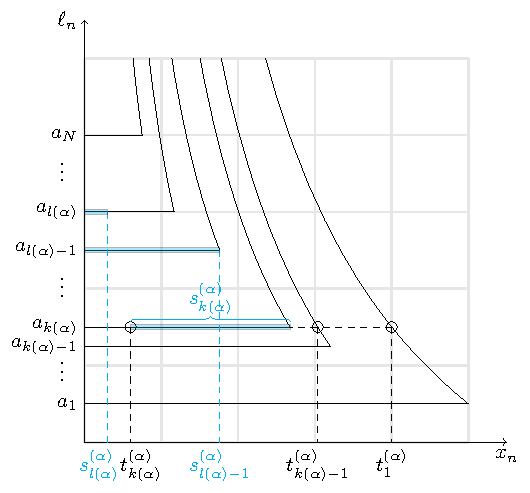
\includegraphics[width=3.3in]{TikZ/stack_NCF_new.pdf}
\caption{Illustration of the NCF strategy. The best Nash equilibrium of the non-compliant flow is given by $(\tV^{(\cR)}, \modeV^{(\cR)})$ (circles) and the NCF strategy~$\sV^{(\cR)}$ is highlighted in blue.}
\label{fig:ncf}
\end{figure}

The NCF strategy saturates links one by one starting from~$\lastNC{\cR}$, the last link in the support of $\tV^{(\cR)}$, until the compliant flow $\alpha \demand$ is completely assigned. Fig.~\ref{fig:ncf} gives an illustration of the NCF strategy. The Non-compliant-first strategy is shown to be an optimal Stackelberg strategy in~\cite{krichene12}.

We note that the induced non-compliant equilibrium $( \tV^{(\cR)}, \modeV^{(\cR)} )$ is given by
\begin{align}
\modeV^{(\cR)} &= \big( 1, \dots, 1, \overbracBig{0}{\lastNC{\cR}}, \dots, 0 \big) \label{eq:NCF-ncMode}\\
\tV^{(\cR)} &= \big( \cFlow{1}{\lastNC{\cR}}, \dots, \cFlow{\lastNC{\cR} - 1}{\lastNC{\cR}}, t^{(\cR)}_{\lastNC{\cR}}, 0, \dots, 0 \big) \label{eq:NCF-ncFlow}
\end{align}
the total flow $\flowV^{(\cR)} = \sV^{(\cR)} + \tV^{(\cR)}$ is given by
\begin{multline}
\flowV^{(\cR)} = \big( \cFlow{1}{\lastNC{\cR}}, \dots, \cFlow{\lastNC{\cR} - 1}{\lastNC{\cR}}, \\
\flowMax_{\lastNC{\cR}}, \dots, \flowMax_{\lastStack{\cR} - 1}, 
\flow_{\lastStack{\cR}}, 0, \dots, 0 \big)
\label{eq:NCF-totalFlow}
\end{multline}
where $\flow_{\lastStack{\cR}}$ is simply given by
\[
\flow_{\lastStack{\cR}} = \demand - \sum_{n = 1}^{\lastNC{\cR} - 1} \cFlow{n}{\lastNC{\cR}} - \sum_{n = \lastNC{\cR}}^{\lastStack{\cR} - 1} \flowMax_n
\]
Finally, the latencies are given by
\[
(a_{\lastNC{\cR}}, \dots, \overbracBig{a_{\lastNC{\cR}}}{\lastNC{\cR}}, a_{\lastNC{\cR}+1}, \dots, a_{\NLinks} )
\]
All these results are summarized in Fig.~\ref{fig:ncf}

% !TEX root = stack-thresh.tex

%%%%%%%%%%%%%%%%%%%%%%%%%%%%%%%%%%%%%%%%%%%%%%%%%%%%%%%%%%%%%%%%%%%%%%%%%%%%%%%%
\section{Supports of equilibria induced by the NCF strategy}
\label{sec:support}

In this section, we show some properties of the supports of the non-compliant equilibrium and the Stackelberg equilibrium induced by the NCF strategy. We consider Stackelberg instances with a fixed number of links~$\NLinks$, a fixed demand~$\demand$, and a variable compliance rate~$\compRate$. Let $\sV^{(\cR)} = \stdStack \NCF$ be the NCF strategy as defined in equation~\eqref{eq:NCF}, $(\tV^{(\cR)}, \modeV^{(\cR)}) = (\tV(\sV^{(\cR)}), \modeV(\sV^{(\cR)}))$ the induced equilibrium of the non-compliant flow as defined in Equations~\eqref{eq:NCF-ncMode} and~\eqref{eq:NCF-ncFlow}, and $\flowV^{(\cR)} = \sV^{(\cR)} + \tV^{(\cR)}$ the total flow of the Stackelberg equilibrium as defined in equation~\eqref{eq:NCF-totalFlow}.

\vspace{5pt}
\begin{definition}
We denote by $\lastStack{\cR}$ the last link in the support of the Stackelberg equilibrium induced by the NCF strategy\footnote{In fact, it is shown in~\cite{krichene12} that any optimal Stackelberg strategy induces the same Stackelberg equilibrium~$\flowV^{(\cR)}$ as the NCF strategy.}, i.e.
\begin{equation}
\lastStack{\cR} = \max \Supp{\flowV^{(\cR)}}
\label{eq:lastStack}
\end{equation}
\end{definition}

\vspace{5pt}
\begin{definition}
We denote by $\lastNC{\cR}$ the last link in the support of the non-compliant equilibrium induced by the NCF strategy, i.e.
\begin{equation}
\lastNC{\cR} = \max \Supp{\tV^{(\cR)}}
\label{eq:lastNC}
\end{equation}
\end{definition}


%-----------------------------------------------------------------------------------------------------------------------------------------------------------------
\subsection{Properties of $\lastNC{\cR}$}

By definition, $(\tV^{(\cR)}, \modeV^{(\cR)})$ is the best Nash equilibrium for the instance $(\NLinks, (1-\compRate)\demand)$. Thus by Proposition~\ref{prop:lastNash}, the last link in its support is also given by
\begin{align}
\lastNC{\cR}
& = \min \left\{k: (1-\compRate)r \leq \demandMax{k} \right\}
\label{eq:lastNC2}
\end{align}

\begin{remark}
\label{rem:max}
We observe that $\demandMax{\lastNC{\cR}} > \demandMax{\lastNC{\cR} - 1}$ (otherwise $\lastNC{\cR}$ would not be minimal and this would contradict equation~\eqref{eq:lastNC2}), therefore we also have
\begin{equation}
\demandMax{\lastNC{\cR}} = \flowMax_{\lastNC{\cR}} + \sum_{n=1}^{\lastNC{\cR}-1} \cFlow{n}{\lastNC{\cR}}\end{equation}
\end{remark}

\begin{proposition}
\label{prop:lastNC_decreasing}
For all compliance rates $\cR_1 \leq \cR_2$, the best Nash equilibrium of ${ (\NLinks,(1-\compRate_2)\demand) }$ uses at most as many links as the best Nash equilibrium of ${ (\NLinks, (1-\compRate_1)\demand) }$. In other words, $\compRate \mapsto \lastNC{\compRate}$ is non-increasing.
\end{proposition}

\begin{proof}
Let $\cR_1 \leq \cR_2$. We have $\forall k$ such that $(1-\cR_1)\demand \leq \demandMax{k}$, $(1-\compRate_2)\demand \leq (1-\compRate_1)\demand \leq \demandMax{k} $. Thus
\[
\{k: (1-\cR_1)\demand \leq \demandMax{k}\} \subset \{k: (1-\cR_2)\demand \leq \demandMax{k}\}
\] 
Therefore using characterization~\eqref{eq:lastNC2}, we have $ \lastNC{\cR_2} \leq \lastNC{\cR_1}$.
\end{proof}

%-----------------------------------------------------------------------------------------------------------------------------------------------------------------
\subsection{Properties of $\lastStack{\cR}$}

In the next two propositions, we show how the support~$\lastNC{\cR}$ of the non-compliant equilibrium affects the support $\lastStack{\cR}$ of the NCF strategy.

\begin{proposition}
\label{prop:lastStack_constant}
For two given compliance rates, $\cR_1$ and~$\cR_2$, if the best Nash equilibria of the instances ${ (\NLinks,(1-\compRate_1)\demand) }$ and ${ (\NLinks, (1-\compRate_2)\demand) }$ have the same support, then the Stackelberg equilibria induced by the NCF strategy for the instances $(\NLinks, \demand, \compRate_1)$ and $(\NLinks, \demand, \compRate_2)$ have the same support. In other words,
\[
\lastNC{\cR_1} = \lastNC{\cR_2} \Rightarrow \lastStack{\cR_1}=\lastStack{\cR_2}
\]
Additionally, we have $\flowV^{(\cR_1)} = \flowV^{(\cR_2)}$.
\end{proposition}

\begin{proof}
Let $\cR_1, \cR_2 \in [0,1]$ be two compliance rates such that $\lastNC{\cR_1} = \lastNC{\cR_2} = k$, and suppose by contradiction that $\lastStack{\cR_1} \neq \lastStack{\cR_2}$. We assume without loss of generality that $\lastStack{\cR_2} > \lastStack{\cR_1}$. The total flow assignments $\flowV^{(\cR_1)}$ and $\flowV^{(\cR_2)}$ both sum to $\demand$, thus we have from the expression~\eqref{eq:NCF-totalFlow} of the total flows
\begin{align}
\demand & = \demandMax{k} + \sum_{n=k+1}^{\lastStack{\cR_1}} \flowMax_n + \flow^{(\cR_1)}_{\lastStack{\cR_1}} \label{prop:lastStack_constant-1}\\
 &= \demandMax{k} + \sum_{n = k+1}^{\lastStack{\cR_2}} \flowMax_n + \flow^{(\cR_2)}_{\lastStack{\cR_2}} \label{prop:lastStack_constant-2}
\end{align}
Substracting~\eqref{prop:lastStack_constant-1} from~\eqref{prop:lastStack_constant-2}, we have
\[
\left( \sum_{n = \lastStack{\cR_1}+1}^{\lastStack{\cR_2}-1} \flowMax_n \right) + \left( \flowMax_{\lastStack{\cR_1}} - \flow^{(\cR_1)}_{\lastStack{\cR_1}} \right) + \flow^{(\cR_2)}_{\lastStack{\cR_2}} = 0
\]
Since every term in the sum is non-negative, all terms are zero. In particular, $\flow^{(\cR_2)}_{\lastStack{\cR_2}} = 0$ which contradicts the definition of $\lastStack{\cR_2}$ as the last link in the support of the Stackelberg equilibrium.
Therefore we have $\lastStack{\cR_2} = \lastStack{\cR_1}$. Finally, we observe from the expression~\eqref{eq:NCF-totalFlow} that~$\flowV^{(\cR)}$ is entirely determined by $\lastNC{\cR}$ and~$\lastStack{\cR}$. This proves that $\flowV^{(\cR_1)} = \flowV^{(\cR_2)}$.
\end{proof}



\begin{proposition}
\label{prop:lastStack}
Let $\cR_1, \cR_2 \in [0,1]$. Then we have
\[
\lastNC{\cR_1} > \lastNC{\cR_2} \Rightarrow \lastStack{\cR_1} \geq \lastStack{\cR_2}
\]
\end{proposition}

\begin{proof}
Let $\cR_1, \cR_2 \in [0,1]$ be two compliance rates such that $\lastNC{\cR_1} > \lastNC{\cR_2}$, and suppose by contradiction that $\lastStack{\cR_1} < \lastStack{\cR_2}$. The total flow assignments $\flowV^{(\cR_1)}$ and $\flowV^{(\cR_2)}$ are given by
\begin{multline*}
\flowV^{(\cR_1)} = \big( \cFlow{1}{\lastNC{\cR_1}}, \dots, \cFlow{\lastNC{\cR_1} - 1}{\lastNC{\cR_1}}, \\
\flowMax_{\lastNC{\cR_1}}, \dots, \flowMax_{\lastStack{\cR_1} - 1}, 
s_{\lastStack{\cR_1}}, 0, \dots, 0 \big)
\end{multline*}
\begin{multline*}
\flowV^{(\cR_2)} = \big( \cFlow{1}{\lastNC{\cR_2}}, \dots, \cFlow{\lastNC{\cR_2} - 1}{\lastNC{\cR_2}}, \\
\flowMax_{\lastNC{\cR_2}}, \dots, \flowMax_{\lastStack{\cR_2} - 1}, 
s_{\lastStack{\cR_2}}, 0, \dots, 0 \big)
\end{multline*}
Since the congestion flow $\cFlow{n}{k}$ is a decreasing function of $k$, and since $\lastNC{\cR_1} > \lastNC{\cR_2}$, we have ${ \forall n \in \{ 1, \dots, \lastNC{\cR_2} - 1\} }$, ${ \cFlow{n}{\lastNC{\cR_1}} < \cFlow{n}{\lastNC{\cR_2}} }$, i.e.
\begin{equation}
\forall n \in \{ 1, \dots, \lastNC{\cR_2} - 1\}, \ \flow_n^{(\cR_1)} <  \flow_n^{(\cR_2)} 
\label{eq:lastStack-proof-1}
\end{equation}
we also have $\forall n \in \{ \lastNC{\cR_2}, \dots, \lastStack{\cR_1} \}$, $\flow_n^{(\cR_2)} = \flowMax_n$, thus by definition of the maximum flow, 
\begin{equation}
\forall n \in \{ \lastNC{\cR_2}, \dots, \lastStack{\cR_1} \}, \ \flow_n^{(\cR_1)} \leq \flow_n^{(\cR_2)}
\label{eq:lastStack-proof-2}
\end{equation}
Summing inequalities~\eqref{eq:lastStack-proof-1} and~\eqref{eq:lastStack-proof-2}, we have
\[
\sum_{n = 1}^{\lastStack{\cR_1}} \flow_n^{(\cR_1)} < \sum_{n = 1}^{\lastStack{\cR_1}} \flow_n^{(\cR_2)}
\]
but $\sum_{n = 1}^{\lastStack{\cR_1}} \flow_n^{(\cR_1)} = \demand$, and $\sum_{n = 1}^{\lastStack{\cR_1}} \flow_n^{(\cR_2)} \leq \sum_{n = 1}^{\lastStack{\cR_2}} \flow_n^{(\cR_2)} = \demand$. This leads to a contradiction and completes the proof.
\end{proof}


\begin{lemma}
\label{lem:lastStack_decreasing}
For all compliance rates $\cR_1 \leq \cR_2$, the Stackelberg equilibrium induced by~$\sV^{(\cR_2)}$ uses at most as many links as the Stackelberg equilibrium induced by~$\sV^{(\cR_1)}$. In other words, $\cR \mapsto \lastStack{\cR}$ is non-increasing.
\end{lemma}
\begin{proof}
This follows from Propositions~\ref{prop:lastNC_decreasing},~\ref{prop:lastStack_constant}, and~\ref{prop:lastStack}.
\end{proof}

\begin{corollary}
\label{corollary:StackVSNash}
The best Stackelberg assignment uses at most as many links as the Best Nash equilibrium, i.e. ${ \lastStack{\cR} \leq \lastNC{0} }$, for any $\cR \in [0,1]$.
\end{corollary}
\begin{proof}
In Stackelberg instance $(\NLinks, \demand, 0)$, since there is no compliant flow to assign, the last link in the support of the total flow $\flowV^{(0)}$ is the last link in the support of the non-compliant flow $\tV^{(0)}$, i.e. $\lastStack{0} = \lastNC{0}$, and since $\cR \geq 0$, we have $\lastStack{\cR} \leq \lastStack{0}$ by Lemma~\ref{lem:lastStack_decreasing}. This completes the proof.
\end{proof}

This corollary states that increasing the compliance rate not only improves the system-wide cost, but it may also allow the central coordinator to use less infrastructure.



% !TEX root = stack-thresh.tex


%%%%%%%%%%%%%%%%%%%%%%%%%%%%%%%%%%%%%%%%%%%%%%%%%%%%%%%%%%%%%%%%%%%%%%%%%%%%%%%%
\section{The cost of Stackelberg equilirbia}
\label{sec:cost}

As in the previous section, we consider Stackelberg instances with a fixed number of links, fixed demand, and variable compliance rate. We derive the analytical expression of the optimal Stackelberg cost,  which we will denote by $C_{\textup{NCF}}(\cR)$, as a function of the compliance rate $\compRate \in [0,1[$\footnote{We exclude the case where the coordinator has total control ($\compRate = 1$) to simplify the discussion: in this case the non-compliant flow is zero and the last link in its support, $\lastNC{1}$ is not defined. The analysis in this case needs a slightly different notation.}. Since the NCF strategy~$\sV^{(\cR)}$ is an optimal Stackelberg strategy, the optimal Stackelberg cost is simply given by
\begin{align}
C_{\textup{NCF}}(\cR) 
&= C(\sV^{(\cR)} + \tV^{(\cR)}, \modeV^{(\cR)})\\
&= C(\flowV^{(\cR)}, \modeV^{(\cR)})\\
&= \sum_{n=1}^{\lastStack{\cR}} \flow^{(\cR)} \latency_n(\flow^{(\cR)}, \mode^{(\cR)}) \label{eq:stackCost}
\end{align}
The main result is that $C_{\textup{NCF}}(\cR)$ is a non-increasing, piecewise-constant function of $\cR$ with discontinuities exactly at the points $\left\{1- \frac{ \maxR{j} }{ \demand } \right\}_{1 \leq j < j_0}$ where $k_j$ are the links that strictly increase the maximum demand, as defined in Section~\ref{sec:previous-Nash}, and $j_0$ is such that the last link in the support of the best Nash equilibrium $\std \BNE$ is $\lastNC{0} = k_{j_0}$.\\

We define intervals $I_1, \dots, I_{j_0}$ as follows:
\begin{itemize}
\item $I_1 = \left[1- \frac{\maxR{1}}{\demand}, 1\right[ = \left[1- \frac{\demandMax{1}}{\demand}, 1\right[$
\item For $1 < j \leq j_0$, ${ I_j = \left[ 1- \frac{\maxR{j}}{\demand}, 1- \frac{\maxR{j-1}}{\demand} \right[ }$
\end{itemize}

\begin{proposition}
\label{prop:j_0}
The interval $I_{j_0}$ satisfies $0 \in I_{j_0}$.
\end{proposition}

\begin{proof}
By~\eqref{eq:lastNC2}, we have
\[
k_{j_0} = \lastNC{0} = \min \{k : \demand \leq \demandMax{k}\}
\]
thus $\demand \leq \demandMax{k_{j_0}}$ and $\demand > \demandMax{k_{j_0 - 1}}$, i.e.
$1 - \frac{\demandMax{k_{j_0}}}{\demand} \leq 0$ and $1 - \frac{\demandMax{k_{j_0 - 1}}}{\demand} > 0$.

\end{proof}

Note that the intervals are disjoint by definition, and by Proposition~\ref{prop:j_0}, ${ [0, 1] \subset I_{j_0} \cup \dots \cup I_1 }$. See Fig.~\ref{fig:intervals} for an illustration of the intervals $\{ I_j \}_{1 \leq j \leq j_0}$.

\begin{figure}[h]
\centering
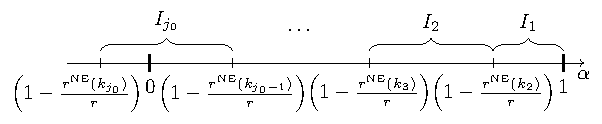
\includegraphics[width=3.4in]{TikZ/intervals.pdf}
\caption{Intervals $\{ I_j \}_{1 \leq j \leq j_0}$.}
\label{fig:intervals}
\end{figure}

First, we prove that on each interval $I_j$, the optimal Stackelberg cost is constant. 

From the expression~\eqref{eq:NCF-totalFlow} of the total flow $\flowV^{(\cR)}$ and the expression~\eqref{eq:NCF-ncMode} of the congestion states, the optimal Stackelberg cost is given by
\begin{multline}
C_{\textup{NCF}}(\compRate) = 
\bigg( \sum_{n = 1}^{\lastNC{\compRate} - 1} \cFlow{n}{\lastNC{\compRate}} \bigg) a_{\lastNC{\compRate}} + \\
\bigg( \sum_{n = \lastNC{\compRate}}^{\lastStack{\compRate} - 1} \flowMax_n a_n\bigg) + 
\flow^{(\cR)}_{\lastStack{\compRate}} a_{\lastStack{\compRate}}
\label{eq:cost}
\end{multline}

In this expression, several terms appear to depend on $\cR$: $\lastNC{\cR}$, $\lastStack{\cR}$ and $\flow^{(\cR)}_{\lastStack{\cR}}$. However, we show that when $\compRate \in I_j$, these terms are constant.
%


\begin{lemma}
\label{lem:cost}
Let $j \in \{1, \dots, j_0 \}$. Then $\forall \compRate \in I_j$, $\lastNC{\cR}$ is constant and equal to $k_j$, $\lastStack{\cR}$ is constant, and the optimal Stackelberg cost $C_{\textup{NCF}}(\cR)$ is constant.
\end{lemma}

\begin{proof}
Let $j \in \{1, \dots, j_0\}$ and let $\compRate \in I_j$. We first show that $\lastNC{\cR} = k_j$. 

For $j \in \{1, \dots, j_0\}$, we have by definition of $I_j$
\[
\compRate \in I_j \Leftrightarrow \demandMax{k_{j-1}} < (1-\compRate)\demand \leq  \demandMax{k_j}
\]
(by convention, we let $k_0 = 0$ and $\demandMax{0} = 0$ so that this statement is true for $j=1$). By the inductive definition~\eqref{eq:nj} of $k_j$, we have $\forall n < k_j$, $\demandMax{n} \leq \demandMax{k_{j-1}}$, thus $\forall n < k_j$, $\demandMax{n} < (1-\compRate)\demand$. Therefore $k_j$ is the minimal index such that $(1-\compRate)\demand \leq \demandMax{k_j}$, i.e. $k_j = \lastNC{\compRate}$ by characterization~\eqref{eq:lastNC}.


Next, since $\lastNC{\compRate}$ is constant, so are $\lastStack{\compRate}$ and $\flowV^{(\cR)}$ by Proposition~\ref{prop:lastStack_constant}. Finally, from~\eqref{eq:cost} the optimal Stackelberg cost is constant since all terms are constant.
\end{proof}

For $\compRate \in I_j$, we will denote by $l_j$ the constant value of $\lastStack{\cR}$, and by $C_j$ the constant value of $C_{\textup{NCF}}(\compRate)$. Note that $l_j$ is by definition
\begin{equation}
\label{eq:l_j}
l_j = \max \bigg\{ l : \demand - \bigg( \maxR{j} + \sum_{n=k_j+1}^{l-1}{\flowMax_n} \bigg) > 0 \bigg\}
\end{equation}


As a consequence of the previous Lemma, the optimal Stackelberg cost is piecewise constant as a function of the compliance rate $\cR$. The next theorem shows that it is a non-increasing function and specifies points of discontinuity.

\begin{theorem}{\emph{Optimal Stackelberg cost}\\}
\label{thm:cost}
The optimal Stackelberg cost $C_{\textup{NCF}}(\alpha)$ is a non-increasing, piecewise-constant function of $\cR \in [0,1[$ with discontinuities exactly at the points $\left\{ 1- \frac{\maxR{j}}{\demand} \right\}_{1 \leq j < j_0}$. On each $I_j$, ${ 1 \leq j \leq j_0 }$, its constant value $C_j$ is given by
\begin{multline}
C_j = 
\bigg( \sum_{n = 1}^{k_j - 1} \cFlow{n}{k_j} \bigg) a_{k_j} + 
\bigg( \sum_{n = k_j}^{l_j - 1} \flowMax_n  a_n \bigg)+ \\
\bigg[\demand - \sum_{n = 1}^{k_j - 1} \cFlow{n}{k_j} - \sum_{n = k_j}^{l_j-1}{\flowMax_n} \bigg] a_{l_j}
\end{multline}
where $l_j$ is given by \eqref{eq:l_j}.
\end{theorem}
\begin{proof}
We need to prove that if $j > i$, then $C_j > C_i$. Let $i, j \in \{1, \dots, j_0 - 1\}$, such that $j > i$ and let $\compRate_i \in I_i$ and $\compRate_j \in I_j$.

We have by Lemma~\ref{lem:cost}, $\lastNC{\cR_i} = k_i$ and $\lastNC{\cR_j} = k_j$. We also have
\begin{itemize}
\item $k_i<k_j$ (since $i<j$)
\item $l_i \leq l_j$ (we have by definition of $I_i$ and $I_j$, $\compRate_i > \compRate_j$, thus by Lemma~\ref{lem:lastStack_decreasing}, $\lastStack{\cR_i} \leq \lastStack{\cR_j}$)
\item $l_i > k_i$ (we have by definition $l_i \geq k_i$. If we have equality, then we have a single-link-free-flow equilibrium supported on $\{1, \dots, k_i\}$, thus $\demand \leq \maxR{i}$, but $k_i < k_j \leq k_{j_0} = \min \{ k | \demand \leq \demandMax{k} \} $, contradiction).
\end{itemize}

We now use the expression~\eqref{eq:NCF-totalFlow} to compare the flows $\flowV^{(\cR_i)}$ and~$\flowV^{(\cR_j)}$.

First, we have $\forall n \in \{1, \dots, k_i-1\}$, $\flow_n^{(\cR_i)} = \cFlow{n}{k_i}$ and $\flow_n^{(\cR_j)} = \cFlow{n}{k_j}$ and since $k_i < k_j$, we have $\cFlow{n}{k_i} > \cFlow{n}{k_j}$ ($\cFlow{n}{\cdot}$ is decreasing). The latencies are given by $\latency_n(\flow_n^{(\cR_j)}, \mode_n^{(\cR_j)}) = a_{k_j}$ and $\latency_n(\flow_n^{(\cR_i)}, \mode_n^{(\cR_i)}) = a_{k_i}$. Thus
\begin{multline}
\forall n \in \{1, \dots, k_i - 1\},
\flow_n^{(\cR_i)} > \flow_n^{(\cR_j)} > 0 \text{ and } \\ 
\latency_n(\flow_n^{(\cR_j)}, \mode_n^{(\cR_j)}) > \latency_n(\flow_n^{(\cR_i)}, \mode_n^{(\cR_i)})
\label{eq:thm_proof_1}
\end{multline}

Second, we have for $n = k_i$, $\flow_{k_i}^{(\cR_i)} = \flowMax_{k_i} $ (since $l_i > k_i$) and $\flow_{k_i}^{(\cR_j)} = \cFlow{n}{k_j}$ (since $k_i < k_j$). Therefore
\begin{equation}
\flow_{k_i}^{(\cR_i)} > \flow_{k_i}^{(\cR_j)} > 0  
\label{eq:thm_proof_2}
\end{equation}

Third, we have $\forall n \in \{k_i, \dots, l_i-1\}$, $\flow_n^{(\cR_i)} = \flowMax_n$, and $\latency_n(\flow_n^{(\cR_i)}, \mode_n^{(\cR_i)}) = a_n$. By definition of the maximum flow, we have $\flow_n^{(\cR_j)} \leq \flowMax_n$, and by definition of the free-flow latency $a_n$, $\latency_n(\flow_n^{(\cR_j)}, \mode_n^{(\cR_j)}) \geq a_n$. Thus
\begin{multline}
\forall n \in \{k_i, \dots, l_i - 1\}, \flow_n^{(\cR_i)} \geq \flow_n^{(\cR_j)} \text{ and } \\
\latency_n(\flow_n^{(\cR_j)}, \mode_n^{(\cR_j)}) \geq \latency_n(\flow_n^{(\cR_i)}, \mode_n^{(\cR_i)})
\label{eq:thm_proof_3}
\end{multline}

Finally, we have $\forall n \in \{l_i, \dots, l_j\}$, $\latency_n(\flow_n^{(\cR_j)}, \mode_n^{(\cR_j)}) \geq a_n$ by definition of the latency function, and $a_n \geq a_{l_i}$ (by the ordering of the links). Thus
\begin{equation}
\forall n \in \{l_i, \dots, l_j\}, \latency_n(\flow_n^{(\cR_j)}, \mode_n^{(\cR_j)}) \geq a_{l_i}
\label{eq:thm_proof_4}
\end{equation}

Using the expression~\eqref{eq:stackCost} of the optimal Stackelberg cost, we have
\begin{align}
C_j 
&= \sum_{n = 1}^{l_j} \flow_n^{(\cR_j)} \latency_n(\flow_n^{(\cR_j)}, \mode_n^{(\cR_j)}) \notag \\
&= \sum_{n = 1}^{l_i-1} \flow_n^{(\cR_j)} \latency_n(\flow_n^{(\cR_j)}, \mode_n^{(\cR_j)}) + 
\sum_{n = l_i}^{l_j} \flow_n^{(\cR_j)} \latency_n(\flow_n^{(\cR_j)}, \mode_n^{(\cR_j)}) \notag \\
&\geq \sum_{n = 1}^{l_i-1} \flow_n^{(\cR_j)} \latency_n(\flow_n^{(\cR_j)}, \mode_n^{(\cR_j)}) + 
\bigg(\sum_{n = l_i}^{l_j} \flow_n^{(\cR_j)} \bigg) a_{l_i} \label{eq:thm_proof_5}\\
&> \sum_{n = 1}^{l_i-1} \flow_n^{(\cR_j)} \latency_n(\flow_n^{(\cR_i)}, \mode_n^{(\cR_i)}) + 
\bigg(\sum_{n = l_i}^{l_j} \flow_n^{(\cR_j)} \bigg) a_{l_i} \label{eq:thm_proof_6}
\end{align}
where inequality~\eqref{eq:thm_proof_5} follows from~\eqref{eq:thm_proof_4}, and inequality~\eqref{eq:thm_proof_6} follows from the fact that ${ \forall n \in \{1, \dots, l_i - 1\} }$,  ${ \flow_n^{(\cR_j)}\latency_n(\flow_n^{(\cR_j)}, \mode_n^{(\cR_j)}) \geq \flow_n^{(\cR_j)}\latency_n(\flow_n^{(\cR_i)}, \mode_n^{(\cR_i)}) }$, with strict inequality for $n \leq k_i$ by~\eqref{eq:thm_proof_1},~\eqref{eq:thm_proof_2} and~\eqref{eq:thm_proof_3}.

We then use the fact that $l_j$ is the last link in the support of $\flowV^{(\cR_j)}$, thus $\demand = \sum_{n = 1}^{l_j} \flow_n^{(\cR_j)}$, i.e.
\[
\sum_{n = l_i}^{l_j} \flow_n^{(\cR_j)} = \demand - \sum_{n = 1}^{l_i - 1} \flow_n^{(\cR_j)}
\]
plugging this in the previous inequality, we have
\begin{align*}
C_j 
&> \bigg( \sum_{n = 1}^{l_i-1} \flow_n^{(\cR_j)} \big( \latency_n(\flow_n^{(\cR_i)}, \mode_n^{(\cR_i)}) - a_{l_i} \big) \bigg)+ \demand a_{l_i}
\end{align*}
We have $\forall n \in \{1, \dots, l_i - 1\}$, $\latency_n(\flow_n^{(\cR_i)}, \mode_n^{(\cR_i)}) - a_{l_i} \leq 0$, and $\flow_n^{(\cR_j)} - \flow_n^{(\cR_i)} \leq 0$, thus
\[
\flow_n^{(\cR_j)} \big( \latency_n(\flow_n^{(\cR_i)}, \mode_n^{(\cR_i)}) - a_{l_i} \big) \geq 
\flow_n^{(\cR_i)} \big( \latency_n(\flow_n^{(\cR_i)}, \mode_n^{(\cR_i)}) - a_{l_i} \big)
\]
plugging this in the previous inequality and rearranging the terms, we obtain
\begin{align*}
C_j 
&> \bigg( \sum_{n = 1}^{l_i-1} \flow_n^{(\cR_i)} \big( \latency_n(\flow_n^{(\cR_i)}, \mode_n^{(\cR_i)}) - a_{l_i} \big) \bigg)+ \demand a_{l_i} \\
&= \bigg( \sum_{n = 1}^{l_i-1} \flow_n^{(\cR_i)} \latency_n(\flow_n^{(\cR_i)}, \mode_n^{(\cR_i)}) \bigg)+ \bigg( \demand - \sum_{n = 1}^{l_i-1} \flow_n^{(\cR_i)} \bigg) a_{l_i} \\
&= C_i
\end{align*}
which competes the proof.
\end{proof}

% !TEX root = stack-thresh.tex

%%%%%%%%%%%%%%%%%%%%%%%%%%%%%%%%%%%%%%%%%%%%%%%%%%%%%%%%%%%%%%%%%%%%%%%%%%%%%%%%
\section{Stackelberg threshold}
\label{sec:threshold}

Now that we have an exact analytical expression of the total cost of a Stackelberg equilibrium as a function of the compliance rate, it becomes easy to express the Stackelberg threshold, or the minimum compliance rate the leader needs to control in order to achieve a strict improvement.
% By Theorem~\ref{thm:cost}, we know that this compliance rate is also the minimal rate such that the support of the induced equilibrium has strictly less links than the best Nash equilibrium of the total users.

\begin{proposition}
\label{prop:thresh}
The Stackelberg threshold is equal to ${ 1 - \frac{\maxR{j_0-1}}{\demand} }$ where $k_{j_0} = k(0) = \min \{k | \demand \leq \demandMax{k}\}$.
\end{proposition}

\begin{proof}
Let $\compRate^\star$ be the Stackelberg threshold. By definition, $\alpha^\star = \min \left\{ \compRate : C_{\mbox{NCF}}(\cR) < C_{\mbox{NCF}}(0) \right\} $.

By Proposition~\ref{prop:j_0}, we have ${ 0 \in I_{j_0} }$, thus ${ C_{\mbox{NCF}}(0) = C_{j_0} }$. And if $\compRate \in I_j$, then $C_{\mbox{NCF}}(\compRate) = C_j$. Thus ${ \compRate^\star =  \min \left\{ \compRate \in I_j : C_j < C_{j_0} \right\} }$ and by Theorem~\ref{thm:cost},
\[
\compRate^\star = \min \left\{ \compRate \in I_{j_0 - 1} \right\}
\]
Therefore the Stackelberg threshold is simply given by the lower bound of interval $I_{j_0 - 1}$, i.e. $\compRate^\star = 1 - \frac{\maxR{j_0-1}}{\demand}$.
\end{proof}

% !TEX root = stack-thresh.tex

%============================================================================================
\section{Numerical results}
\label{sec:numerical}

In this section, we illustrate the results of Sections~\ref{sec:cost} and~\ref{sec:threshold} by numerically simulating the NCF strategy and computing its cost on an example network.
We generated a network with $\NLinks = 5$ links, and arbitrary latency functions, shown in Fig.~\ref{fig:num_latencies}. 

\begin{figure}[h]
\centering
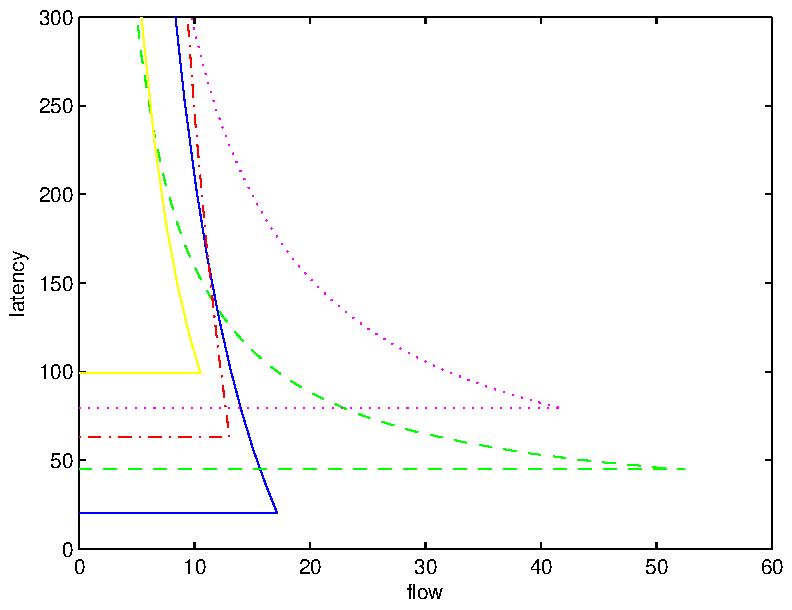
\includegraphics[width = 2.5in]{figures/latencies}
\caption{Latency functions for the example network.}
\label{fig:num_latencies}
\end{figure}

The optimal Stackelberg cost is computed for ${ \demand \in [0, \demandMax{\NLinks}] }$ and $\compRate \in [0,1]$. The results are shown in Fig.~\ref{fig:num_cost}. For a fixed demand, the optimal cost is a piecewise constant function of $\compRate$ (Fig.~\ref{fig:num_cost_2}). This also illustrates the intervals $\{I_j\}_{1 \leq j \leq j_0}$ discussed in the previous section. In this example, we have $\demandMax{1} < \demandMax{2} \leq \demandMax{3} < \demandMax{4} \leq \demandMax{5}$, therefore the links that achieve a strict increase in the capacity are $k_1 = 1$, $k_2 = 2$ and $k_3 = 4$.

\begin{figure}[h]
\centering
\begin{subfigure}[b]{3.3in}
\centering
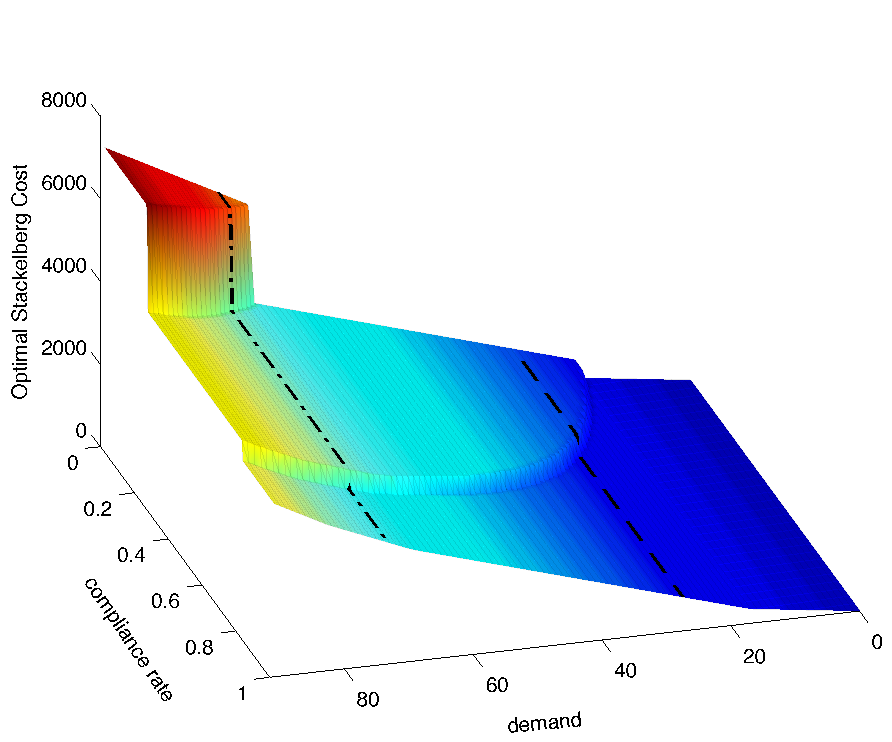
\includegraphics[width=2.8in]{figures/cost_surface}
\caption{Optimal Stackelberg cost as a function of $\demand$ and~$\compRate$. Iso-$\demand$ lines are plotted for $\demand = 0.3 \ \demandMax{\NLinks}$ (dashed) and ${ \demand = 0.8 \ \demandMax{\NLinks} }$ (dot-dashed).}
\label{fig:num_cost_1}
\end{subfigure}

\begin{subfigure}[b]{3.3in}
\vspace{10pt}
\centering
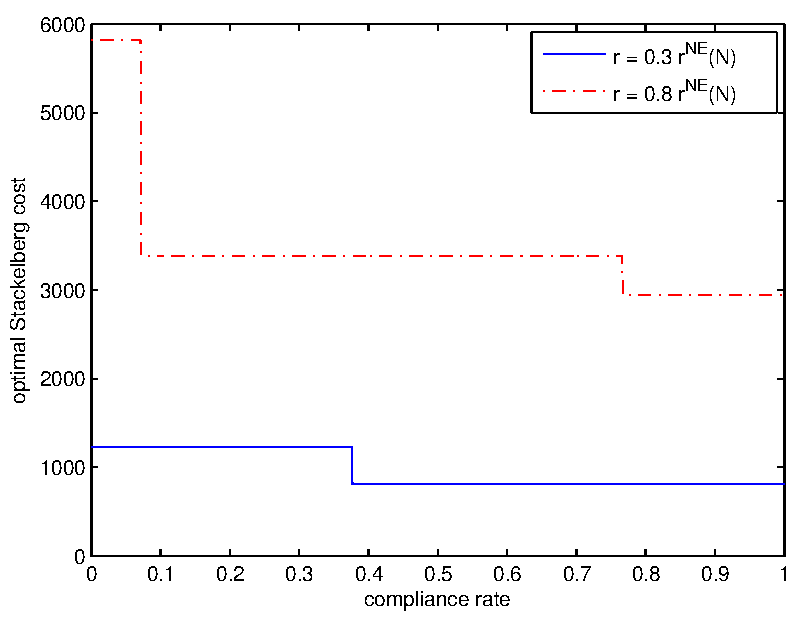
\includegraphics[width=2.6in]{figures/cost}
\caption{$C_{\textup{NCF}}(\compRate)$: optimal Stackelberg cost for a fixed demand $\demand$. The cost is a non-increasing, piecewise constant function of~$\compRate$. When the demand is ${ \demand = 0.8 \ \demandMax{\NLinks} }$, we have $j_0 = 3$, therefore we have two discontinuities, at $1 - \frac{\demandMax{k_1}}{\demand}$ and $1 - \frac{\demandMax{k_2}}{\demand}$.}
\label{fig:num_cost_2}
\end{subfigure}

\caption{Optimal Stackelberg cost.}
\label{fig:num_cost}
\end{figure}


Finally, we numerically compute and plot the Stackelberg threshold for different values of the demand. The results, shown in Fig.~\ref{fig:num_stack_thresh}, match the analytical expression given in Proposition~\ref{prop:thresh}. We observe that for low values of demand ($\demand < \demandMax{1}$), the social optimum and the Nash equilibrium ($\compRate = 0$) are identical, therefore Stackelberg routing cannot strictly improve the cost. For $\demand > \demandMax{1}$, we observe two branches: the first one corresponds to the range of demands $\demand \in ]\demandMax{1}, \demandMax{2}]$, for which the Stackelberg threshold is given by $1-\frac{\demandMax{k_1}}{\demand}$ ($j_0 = 2$, i.e. $k(0) = k_2 = 2$). The second one corresponds to the range of demands $]\demandMax{2}, \demandMax{4}]$, for which the Stackelberg threshold is given by $1-\frac{\demandMax{k_2}}{\demand}$ ($j_0 = 3$, i.e. $k(0) = k_3 = 4$).


\begin{figure}[h]
\centering
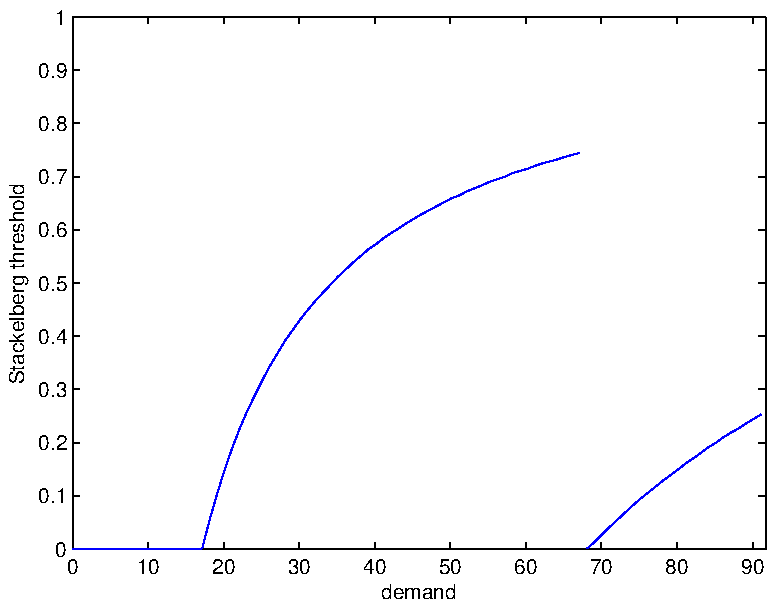
\includegraphics[width = 2.6in]{figures/threshold}
\caption{Stackelberg threshold for increasing values of demand.}
\label{fig:num_stack_thresh}
\end{figure}




% !TEX root = stack-thresh.tex

%%%%%%%%%%%%%%%%%%%%%%%%%%%%%%%%%%%%%%%%%%%%%%%%%%%%%%%%%%%%%%%%%%%%%%%%%%%%%%%%
\section{Discussion and Concluding remarks}
\label{sec:conclusion}

We studied Stackelberg routing games on parallel networks with the HQSF latency class, and we studied, in particular, how the optimal Stackelberg cost depends on the compliance rate $\compRate$. We proved that it is a non-increasing, piecewise constant function, with discontinuities at specific points described in Theorem~\ref{thm:cost}. As a consequence, we obtained an expression for the Stackelberg threshold, i.e. the minimal compliance rate needed to achieve a strict improvement in the cost. These results were illustrated using an example network for which we numerically computed the optimal Stackelberg cost and the Stackelberg thresholds. These results can be useful for efficient planning and control, for example on traffic networks. If a traffic planner can estimate the total demand on a parallel network, they can compute, given a model of latency on each route\footnote{In a traffic setting, it is possible to derive latency functions that satisfy the assumptions of the HQSF class, by considering a triangular fundamental diagram of traffic for example. For a discussion on this topic, see~\cite{krichene12}.}, the compliance rate needed to strictly improve the cost. This Stackelberg threshold can inform the planner whether Stackelberg routing is practical for the network considered.

While these results can be applicable in some scenarios of traffic, the simple topology of parallel networks limits applicability to a small subset of real networks. An immediate question is whether these results extend to more general topologies, and in particular, whether it is simple to characterize an optimal Stackelberg strategy for these topologies (similar to the NCF strategy in the parallel case). A second question is reachability of the equilibria: the analysis presented here gives existence results of static equilibria. Assuming one defines a dynamic model of response of the players to a Stackelberg strategy, a natural question is: which equilibria are reachable, and what are the optimal Stackelberg strategies in the dynamic case?


\addtolength{\textheight}{-12cm}   % This command serves to balance the column lengths
                                  % on the last page of the document manually. It shortens
                                  % the textheight of the last page by a suitable amount.
                                  % This command does not take effect until the next page
                                  % so it should come on the page before the last. Make
                                  % sure that you do not shorten the textheight too much.


%%%%%%%%%%%%%%%%%%%%%%%%%%%%%%%%%%%%%%%%%%%%%%%%%%%%%%%%%%%%%%%%%%%%%%%%%%%%%%%%
\bibliographystyle{plain}
\bibliography{common/bibliography}


\end{document}
